\documentclass[a4paper,12pt]{article}
\usepackage{cmap} % поиск русских слов в полученном pdf-файле
\usepackage[T2A]{fontenc} % Поддержка русских букв
\usepackage[utf8x]{inputenc}
\usepackage{ucs}
\usepackage[english,russian]{babel}
\usepackage{makeidx} % пакет для создания алфавитного указателя
\usepackage{amsthm,amsfonts,amsmath,amssymb,amscd} % эти пакеты необходимы для набора формул
\usepackage{graphicx}
\usepackage{indentfirst}% Красная строка в первом абзаце
\usepackage{tabularx}
\usepackage[labelsep=period]{caption} % пакет для управления заголовка рисунков и таблиц
\usepackage{subfig} % пакет для расположения нескольких под рисунков в одном окружении figure
\usepackage{longtable}
\usepackage{cite}

\usepackage{geometry} % Меняем поля страницы
\geometry{left=3cm}% левое поле
\geometry{right=2cm}% правое поле
\geometry{top=2cm}% верхнее поле
\geometry{bottom=2cm}% нижнее поле
\sloppy % Избавляемся от переполнений
\clubpenalty=10000 % Запрещаем разрыв страницы после первой строки абзаца
\widowpenalty=10000 % Запрещаем разрыв страницы после последней строки абзаца
\newcommand{\includepic}[2][]{\includegraphics[#1]{#2.png}}
%
\linespread{1.3} % интервал
\graphicspath{{fig/}}

\makeindex % сделаем именной указатель, но печатаем его отдельной командой(если печатаем)
\frenchspacing %пробел после запятой не увеличивается - так принято в России
\righthyphenmin=2 % можно оставлять два символа на строке при переносе

%%==========================================================================================
\begin{document}
\pagenumbering{arabic}
\numberwithin{equation}{section}
\renewcommand{\theequation}{\thesection.\arabic{equation}}

\begin{titlepage}
\begin{center}

{\bf Ордена Ленина \\
ИНСТИТУТ ПРИКЛАДНОЙ МАТЕМАТИКИ \\
имени М.В.~Келдыша \\
Российской академии наук \\
\par}

\vspace{50mm}

{\bf \large А.А.~Люпа, Е.Б.~Савенков\par}

\vspace{10mm}

{\bf \Large Модель двухфазной фильтрации с~релаксацией потока
и анализ эффективности применения явных схем
\par}

\end{center}

\vspace{\fill}

\begin{center}
{\bf Москва --- 2016}
\end{center}

\clearpage
\end{titlepage}
\newpage

{\noindent \textit{ \textbf {Люпа~А.А., Савенков~Е.Б.}}}


{\bf Модель двухфазной фильтрации \\ с~релаксацией потока \\
и анализ эффективности применения явных схем} \\


В работе рассматривается модификация классической модели
изотермической двухфазной фильтрации в пористых средах, полученная 
введением релаксации потока в уравнениях неразрывности.
Представлены результаты численного исследования предложенной модели,
а также применения явных численных методов со сниженным ограничением на
шаг по времени. \\


{\textit{ \textbf {Ключевые слова:}}} течение жидкости в пористой среде, явные конечно-разностные схемы \\ \\ \\


{\noindent \textit{ \textbf { Anastasiya Alexandrovna Lyupa, Evgeny Borisovich Savenkov}}}


{\bf Two-phase flow model with flow relaxation
and effectiveness analysis of the explicit schemes application} \\


The paper focuses on the modification of the classical model of isothermal two-phase 
flow in porous media by addition of flow relaxation to the continuity equation. 
The results of a numerical study of the proposed model are presented. 
Explicit numerical methods with a reduced restriction on time step are applied. \\


{\textit{ \textbf {Key words and phrases:}}} fluid flow in a porous medium, explicit finite difference schemes \\ \\ \\


Работа выполнена при поддержке Российского фонда фундаментальных исследований, проекты 16-29-15095-офи\_м, 15-01-03445-а, 15-01-03654-а. \\ \\ \\

\tableofcontents
\newpage

\section{Введение}
Теория фильтрации, изучающая законы движения жидкостей, газов и их смесей в
пористой среде, имеет обширное практическое применение. На протяжении многих лет
фильтрационные расчеты занимают очень важное место при разработке технологий
добычи нефти и газа, при проектировании, постройке и эксплуатации
гидротехнических  и мелиоративных сооружений, в горном деле, в решении
экологических проблем. В настоящее время, с появлением мощных расчётных систем,
обладающих возможностями обрабатывать огромные объемы информации, задачи фильтрации
становятся все более и более актуальными.

Настоящая работа посвящена проблемам, связанным с течениями трехфазной жидкости 
сквозь пористую среду. Процессы напрямую зависят от свойств почв, их неоднородности. 
Три рассматриваемые фазы: вода, газ и NAPL(от английского Non-Aqueous Phase 
Liquids). К NAPL, например, относятся минеральное топливо, растворители, очищающие средства. 
В зависимости от того, как соотносится плотность вещества с плотностью воды, 
NAPL разделяются на легкие и плотные (первые называются Light NAPL, или LNAPL, их плотность меньше плотности
воды; вторые - Dense NAPL, или DNAPL, соответственно их плотность больше
плотности воды). Бензин, например, относится к первому типу, а тетрахлороэтилен
- ко второму. Эти жидкости не смешиваются с водой и с газом, поэтому при моделировании их течения
в почве говорят  о многофазной фильтрации.

Основной целью работы является получение распределения насыщенностей и давлений
трех фаз в пласте среды в зависимости от времени, начальных и граничных
условий, свойств и неоднородностей почв. 

Численные решения таких задач, также как и других задач газо- и гидродинамики,
требуют больших вычислительных затрат. В то же время существует необходимость в
наиболее быстром получении результатов. Использование
высокопроизводительных параллельных компьютеров с распределенной памятью
позволяет проводить вычисления в течение разумного времени. Поэтому созданные
вычислительные алгоритмы были адаптированы к расчетам на многопроцессорных
вычислительных комплексах. Для вычислений используются стандартная
библиотека MPI и технология Nvidia CUDA(для задействования в расчетах 
высокопроизводительных графических плат). При расчетах применяются явные разностные 
схемы, допускающие эффективное распараллеливание. Вычисления проводятся
на гибридном вычислительном комплексе K-100, ИПМ им. М.В.Келдыша РАН.

%
\section{Физическое описание задачи}
%
%
	Законы движения флюидов в пористых средах базируются на сохранении
массы, энергии, импульса. С практической точки зрения безнадежно в настоящее
время приложить эти законы непосредственно к рассматриваемым задачам. Основные
физические свойства пористой среды могут быть связаны с элементарным
объемом среды, который должен быть достаточно большим по сравнению с размером
пор. Подземные пространства характеризуются сложной системой пор, каналов,
трещин, размеры которых малы по сравнению с характерными размерами среды, и по
которым может происходить течение жидкости или газа. Количественной
характеристикой пористости среды
служит отношение объема пор к общему объему:
%
	$$m=V_n/V,$$
%	 	
где $m$ -- коэффициент пористости, $V_n$ -- объем пор, $V$ -- общий объем
данного
элемента среды.
%
Течение через такие пористые тела, при котором сила трения флюида
(жидкости, газа) о скелет играет определяющую роль, называется фильтрацией.
Часть системы, все компоненты которой имеют
одинаковые физические и химические свойства, называется фазой. 

Главными характеристиками движения многофазной системы являются насыщенности и
скорости фильтрации каждой из фаз. Насыщенностью $S_i$  порового пространства
$i$-ой фазой называется доля объема пор, занятая этой фазой в элементарном
объеме:
%
\begin{equation} 
S_i=\frac{\Delta V_i}{\Delta V}, i=1,2\ldots n,{\quad}\sum_{i=1}^{n}S_i=1. 
\end{equation}
%
Для каждой фазы существует предельная насыщенность, такая, что при меньших
значениях насыщенности эта фаза неподвижна. Эти значения носят название остаточных 
насыщенностей. Обозначаем их с помощью нижнего индекса $r$ у насыщенностей. Таким 
образом, совместное течение двух фаз имеет место лишь в интервале насыщенностей.
Для работы в данном интервале насыщенностей вводится понятие эффективных 
насыщенностей фаз, их обозначаем с помощью символа верхней черты. Эффективная насыщенность 
$i$-ой фазы трехфазной жидкости может быть записана в виде:
$$\overline{S_i}={\frac{S_i-S_{ir}}{1-\sum\limits_{j=1}^{3}S_{jr}}}.$$

Проекция скорости фильтрации $i$-ой фазы в некоторой точке
$\overrightarrow{u_i}$ на некоторое направление равна отношению объемного
расхода данной фазы к площадке, перпендикулярной к указанному направлению.
Основное соотношение теории фильтрации -- закон фильтрации(закон Дарси) -- устанавливает 
связь между вектором скорости фильтрации и тем полем давления, которое вызывает 
фильтрационное течение. Закон Дарси в теории фильтрации заменяет собой уравнение 
движения. Для $i$-ой фазы при учете силы тяжести его можно записать в виде:
\begin{equation}
\label{Darcy}
  \overrightarrow{u_i}=-K \frac{k_i(S_i)}{{\mu}_i}(grad P_i - {\rho}_i\overrightarrow{g}),
\end{equation}
где $K$ -- характеристика пористой среды, называемая
абсолютной проницаемостью, определяемая по данным о фильтрации однородной
жидкости и не зависящая от свойств жидкости; $\mu_i$ -- коэффициент динамической
вязкости $i$-ой фазы ($\mu_i=\mu_i(T)$); $k_i(S_i)$ -- относительная фазовая проницаемость $i$-ой фазы(может зависеть 
не только от насыщенности $i$-ой фазы), определяемые
экспериментально; $P_i$ -- давление в $i$-ой фазе; ${\rho}_i$ -- плотность $i$-ой фазы;
$\overrightarrow{g}$ -- вектор ускорения свободного падения.
Можно выделить верхнюю и нижнюю границы применимости закона Дарси\cite{Bahvalov}. Верхняя граница связана 
с проявлением инерционных сил при достаточно высоких скоростях фильтрации. Нижняя --
с взаимодействием жидкости с твердым скелетом пористой среды при достаточно малых 
скоростях фильтрации.

Еще одно фундаментальное соотношение в теории фильтрации - уравнение неразрывности. 
Для $i$-ой фазы оно принимает вид:
 \begin{equation}
 \label{mass}
 	 \frac{\partial (m \rho_i S_i)}{\partial t}+ div(\rho_i \overrightarrow{u_i}) = \rho_i q_i.
 \end{equation}
В отсутствие объемных источников $i$-ой фазы
соответсвующее слагаемое в правой части уравнения (${\rho_i}q_i$) обнуляется.

При малых размерах области фильтрации и малых скоростях капиллярные силы могут
превзойти внешний перепад давления, и их необходимо учитывать.
Капиллярные эффекты обусловлены межмолекулярными взаимодействиями двух различных
фаз. Эти силы приводят к появлению угла смачивания на границе раздела двух фаз и
к разрыву давления на этой границе. Разность фазовых давлений есть так
называемое \textit{капиллярное давление}. Соотношения между капиллярными
давлениями и насыщенностями обычно получают по опытным данным как функции насыщенностей.

Закон сохранения энергии для многофазной системы может быть записан в виде
\begin{equation}
\label{Energy_law}
  \frac{\partial \left(m {\sum\limits_{i}{\rho_i S_i E_i}} + (1-m){\rho_r E_r}\right)}{\partial t}
    + div(\sum_{i}{\rho_i H_i \overrightarrow{u_i}}) = div(\lambda_{eff} grad T),
\end{equation}
где суммирование производится по всем активным фазам, индекс $r$ обозначает твердую породу,
эффективный коэффициент теплопроводности:
\begin{equation}
\lambda_{eff}=m\sum_i{S_i\lambda_i} + (1-m)\lambda_r,
\end{equation}
связь между внутренней энергией $E_i$ и энтальпией $H_i$:
\begin{equation}
E_i=H_i-\frac{P_i}{\rho_i},
\end{equation} для нахождения энтальпии нужно знать зависимость теплоемкости
вещества при постоянном давлении от температуры:
\begin{equation}
H_i=H_{i0}+\int_{T_0}^{T}{C_P(T)dT}.
\end{equation}
Зависимости коэффициентов теплопроводности и теплоемкостей находятся эмпирически.

Для замыкания системы дополнительно вводятся уравнения состояния рассматриваемого флюида
и пористой среды.

%
\section{Математическая модель}
\label{math_section}
%
В работе проводится моделирование трехфазной неизотермической фильтрации 
несмешивающихся жидкостей и газа с учетом их сжимаемости. Скелет породы
считаем неподвижным, пористость и плотность породы -- постоянными во всем
рассматриваемом объеме, среду -- изотропной, жидкие фазы -- слабосжимаемыми,
газ -- идеальным, температуру -- единой для всех фаз.

Рассматриваются одномерные, двумерные и трехмерные
области, заданные в декартовых координатах.

Рассмотрим более детально описанные в главе, посвященной физической
модели, законы и принципы с учетом введенных ограничений и опишем
используемые зависимости физических свойств фаз.

Пусть трехфазная система представляет собой две жидкие фазы -- вода и легкий
нефтяной продукт (LNAPL -- от английского Light Non-Aqueous Phase Liquids,
плотность которого меньше плотности воды), и одну газообразную.
Для удобства введем индексные обозначения для разных фаз: $w$ -- вода, $n$ --
легкая нефть, $g$ -- газ.

В качестве базовых переменных выбираем насыщенности, давления фаз и температуру.
Причем для насыщенностей в силу определения справедливо  $S_w + S_n + S_g = 1$.
А давления $P_n$ и $P_g$ отличаются от $P_w$ на величины капиллярных
давлений, являющихся функциями от насыщенностей.

Вводятся эффективные насыщенности каждой из фаз:
$\overline{S_i}={\dfrac{S_i-S_{ir}}{1-S_{wr}-S_{nr}-S_{gr}}}$, где , ${\quad}i=w,n,g$, $S_{wr}$,
$S_{nr}$, $S_{gr}$ -- остаточные насыщенности фаз.

\subsection{Капиллярные давления на границах фаз}
Для описания
капиллярных давлений выбрана приближенная модель Паркера\cite{Parker}:
$$P_{cnw}(\overline{S_w})=P_n-P_w={\frac{1}{\gamma \delta_{nw}}}
\left( \overline{S_w}^{\frac{n}{1-n}}-1 \right)^\frac{1}{n},\;0<\overline{S_w}<1 $$
$$P_{cgn}(\overline{S_g})=P_g-P_n={\frac{1}{\gamma \delta_{gn}}}
\left( (1-\overline{S_g})^{\frac{n}{1-n}}-1 \right)^\frac{1}{n},\;0<\overline{S_g}<1$$
(где $P_{cnw}(\overline{S_w})$ - и $P_{cgn}(\overline{S_g})$- капиллярные давления на границах вода-нефть и нефть-газ, 
соответственно, $n$ и $\gamma $ -- пареметры породы Ван Генухтена из соответствующего приближения
Ван Генухтена\cite{Genuchten}, $\delta_{nw}$, $\delta_{gn}$ -- коэффициенты, определяемые поверхностным натяжением 
жидкостей). В работе используются следующие значения параметров: $n$ = 3.25, $\gamma $ = 0.00048Па$^{-1}$,
$\delta_{nw}$ = 0.67, $\delta_{gn}$ = 2. Зависимости капиллярных давлений от насыщенностей фаз
изображены на Рис.~\ref{tikz_P_cnw}, Рис.~\ref{tikz_P_cgn}.

\begin{figure}[h]
\begin{minipage}[h]{0.49\linewidth}
\begin{tikzpicture}
  \begin{axis}[grid=major, axis lines=left, enlargelimits=true, width=1\linewidth, xlabel={$\overline{S_w}$}, ylabel={$P_{cnw}$, Па}]
    \addplot[domain=0.001:1.0, samples=100, ultra thick, magenta]{pw(x,3.25,0.00048,0.67)};
  \end{axis}
\end{tikzpicture}
\caption{Зависимость капиллярного давления на граице нефть-вода
$P_{cnw}$ от эффективной насыщенности водной фазы $\overline{S_w}$}
\label{tikz_P_cnw}
\end{minipage}
\hfill
\begin{minipage}[h]{0.49\linewidth}
\begin{tikzpicture}
  \begin{axis}[grid=major, axis lines=left, enlargelimits=true, width=1\linewidth, xlabel={$\overline{S_g}$}, ylabel={$P_{cgn}$, Па}]
    \addplot[domain=0.001:0.999, samples=100, ultra thick, magenta]{pg(x,3.25,0.00048,2.0)};
  \end{axis}
\end{tikzpicture}
\caption{Зависимость капиллярного давления на границе газ-нефть 
$P_{cgn}$ от эффективной насыщенности газовой фазы $\overline{S_g}$}
\label{tikz_P_cgn}
\end{minipage}
\end{figure}

\subsection{Относительные фазовые проницаемости}
Относительные фазовые проницаемости определяются в~ работе в~ соответствии с~
приближением Стоуна\cite{Aziz-Settari}:

\begin{equation*}
  k_{w}(\overline{S_w})=
  \begin{cases}
  &\overline{S_w}^\frac{1}{2} \left( 1-\left( 1-\overline{S_w}^\frac{n}{n-1} \right) ^\frac{n-1}{n} \right) ^2
  \text{ , $0<\overline{S_w}<1$}\\
  &1 \text{ , $\overline{S_w}\ge 1$}\\
  &0 \text{ , $\overline{S_w}\le 0$}
\end{cases} 
\end{equation*}
\begin{equation*}
  k_{g}(\overline{S_g})=
  \begin{cases}
  &\overline{S_g}^\frac{1}{2} \left( 1-\left ( 1-\overline{S_g} \right) ^\frac{n}{n-1} \right) ^\frac{2(n-1)}{n}
  \text{ , $0<\overline{S_g}<1$}\\
  &1 \text{ , $\overline{S_g}\ge 1$}\\
  &0 \text{ , $\overline{S_g}\le 0$}
  \end{cases} 
\end{equation*}
\begin{equation*}
  k_{n}(\overline{S_w},\overline{S_n})=
  \begin{cases}
  &\dfrac{\overline{S_n} k_{nw}(\overline{S_w})k_{ng}(\overline{S_n})}{(1-\overline{S_w})(\overline{S_w}+\overline{S_n})}
  \text{ , $\overline{S_w}<1, \quad \overline{S_w}+\overline{S_n} >0$}\\
  &0 \text{ , иначе}
  \end{cases}\text { , где}
\end{equation*}\\
\begin{equation*}
  k_{nw}(\overline{S_w})=
  \begin{cases}
  &(1-\overline{S_w})^\frac{1}{2} \left(1-\overline{S_w}^\frac{n}{n-1} \right) ^\frac{2(n-1)}{n}
  \text{ , $0<\overline{S_w}<1$}\\
  &1 \text{ , $\overline{S_w}\le 0$}\\
  &0 \text{ , $\overline{S_w}\ge 1$}
  \end{cases}\text { , }
\end{equation*}
\begin{equation*}
  k_{ng}(\overline{S_n})=
  \begin{cases}
  &\overline{S_n}^\frac{1}{2} \left( 1-\left( 1-\overline{S_n}^\frac{n}{n-1} \right) ^\frac{n-1}{n} \right) ^2 
  \text{ , $0<\overline{S_n}<1$}\\
  &1 \text{ , $\overline{S_n}\ge 1$}\\
  &0 \text{ ,  $\overline{S_n}\le 0$}
\end{cases}
\end{equation*}
 
Таким образом, относительные проницаемости воды и~ газа являются функциями одной 
переменной(насыщенности одной из фаз), а нефти -- двух. Данные зависимости
изображены на~ Рис.~\ref{tikz_k_w}, Рис.~\ref{tikz_k_g}, Рис.~\ref{tikz_k_n},
соответственно.

\begin{figure}[h]
\begin{minipage}[h]{0.49\linewidth}
\begin{tikzpicture}
  \begin{axis}[grid=major, axis lines=left, enlargelimits=true, width=1\linewidth, xlabel={$\overline{S_w}$}, ylabel={$k_w$}]
    \addplot[domain=0.0:1.001, samples=100, ultra thick, red]{kw(x,3.25)};
  \end{axis}
\end{tikzpicture}
\caption{Зависимость относительной фазовой проницаемости воды $k_w$
  от эффективной насыщенности водной фазы $\overline{S_w}$}
\label{tikz_k_w}
\end{minipage}
\hfill
\begin{minipage}[h]{0.49\linewidth}
\begin{tikzpicture}
  \begin{axis}[grid=major, axis lines=left, enlargelimits=true, width=1\linewidth, xlabel={$\overline{S_g}$}, ylabel={$k_g$}]
    \addplot[domain=0.0:1.0, samples=100, ultra thick, red]{kg(x,3.25)};
  \end{axis}
\end{tikzpicture}
\caption{Зависимость относительной фазовой проницаемости газа $k_g$ 
  от эффективной насыщенности газовой фазы $\overline{S_g}$}
\label{tikz_k_g}
\end{minipage}
\end{figure}

\begin{figure}[h]
\begin{center}
\begin{tikzpicture}
  \begin{axis}[xtick={0.0,0.2,...,1.0}, ytick={0.0,0.2,...,1.0}, ztick={0.0,0.2,...,1.0}, grid=major, xlabel={$\overline{S_w}$}, ylabel={$\overline{S_n}$}, zlabel={$k_n$}]
    \addplot3[surf, samples=20, domain=0.00:0.99,y domain=0.00:0.99]{kn(x,y)};
  \end{axis}
\end{tikzpicture}
\caption{Зависимость относительной фазовой проницаемости нефти $k_n$ 
  от эффективных насыщенностей водной и нефтяной фаз $\overline{S_w}$ и $\overline{S_n}$}
\label{tikz_k_n}
\end{center}
\end{figure}

\subsection{Теплопроводность, теплоемкость, вязкость}
Коэффициенты теплопроводности фаз представлены зависимостями:
\begin{equation}
  \begin{aligned}
    &\lambda_w(T)=0.553\times(1-0.003\times(T-T_0)),\\
    &\lambda_n(T)=0.14\times(1-0.001\times(T-T_0)),\\
    &\lambda_g(T)=0.237\times\left(\frac{T}{T_0}\right)^{0.82},\\
    &\lambda_r(T)=1.0.
  \end{aligned}
\end{equation}
Теплоемкости фаз при постоянном давлении:
\begin{equation}
  \begin{aligned}
    &C_{Pw}(T)= 4194 - 1.15 \times (T-T_0) + 0.015 \times (T-T_0)^2,\\
    &C_{Pn}(T)= 1700 - 3.4 \times (T-T_0),\\
    &C_{Pg}(T)= 1000 - 0.119 \times (T-T_0),\\
    &C_{Pr}(T)= 800 - 0.75 \times (T-T_0).
  \end{aligned}
\end{equation}

Динамические вязкости фаз (см. Рис.~\ref{tikz_mu_w}, Рис.~\ref{tikz_mu_n}, Рис.~\ref{tikz_mu_g}):
\begin{equation}
  \begin{aligned}
    &\mu_w(T)=\frac{1}{29.21 \times T - 7506.64},\\
    &\mu_n(T)=7.256\times10^{-10} \times e^{\frac{4141.9}{T}},\\
    &\mu_g(T)=1.717\times10^{-5} \times \left(\frac{T}{T_0}\right)^{0.683}.
  \end{aligned}
\end{equation}
Здесь $T_0=273K$.

\begin{figure}[h]
\begin{minipage}[h]{0.49\linewidth}
\begin{tikzpicture}
  \begin{axis}[grid=major, axis lines=left, enlargelimits=true, width=1\linewidth, ylabel={$\mu_w$, Па$\cdot$с}, xlabel={$T$, К}]
    \addplot[domain=275:350, samples=100, ultra thick, blue]{mw(x)};
  \end{axis}
\end{tikzpicture}
\caption{Зависимость вязкости воды $\mu_w$ от температуры}
\label{tikz_mu_w}
\end{minipage}
\hfill
\begin{minipage}[h]{0.49\linewidth}
\begin{tikzpicture}
  \begin{axis}[grid=major, axis lines=left, enlargelimits=true, width=1\linewidth, ylabel={$\mu_n$, Па$\cdot$с}, xlabel={$T$, К}]
    \addplot[domain=275:350, samples=100, ultra thick, blue]{mn(x)};
  \end{axis}
\end{tikzpicture}
\caption{Зависимость вязкости нефти $\mu_n$ от температуры}
\label{tikz_mu_n}
\end{minipage}
\end{figure}

\begin{figure}[h]
\begin{center}
\begin{tikzpicture}
  \begin{axis}[grid=major, axis lines=left, enlargelimits=true, width=0.49\linewidth, ylabel={$\mu_g$, Па$\cdot$с}, xlabel={$T$, К}]
    \addplot[domain=275:350, samples=100, ultra thick, blue]{mg(x)};
  \end{axis}
\end{tikzpicture}
\caption{Зависимость вязкости воздуха $\mu_g$ от температуры}
\label{tikz_mu_g}
\end{center}
\end{figure}

\subsection{Уравнения состояния}
Перейдем к уравнениям состояний фаз.
Водную и нефтяную фазы считаем слабосжимаемыми и линейно зависящими от перепада температуры:\\
$${\rho}_i = {\rho}_{i0} {(1 + {\beta}_i (P_i-P_0) - {\alpha}_i (T-T_0))},
{\quad}0<{\beta}_{i}{\ll}1,{\quad}0<{\alpha}_{i}{\ll}1,{\quad}i=w,n,$$
где ${\rho}_{i0}$ -- известное значение плотности $i$-ой фазы, соответсвующее
значению давления $P_0$ и~ температуры $T_0$.

Для газа предполагаем справедливым уравнение состояния идеального
газа:
$${\rho}_g = {\rho}_{g0}{\frac{P_g}{P_0}}{\frac{T_0}{T}}.$$

В работе используются следующие значения:\\
$\rho_r=2000$ кг/м$^3$, $\rho_{w0}=1000$ кг/м$^3$,
$\rho_{n0}=850$ кг/м$^3$, $\rho_{g0}=1.4$ кг/м$^3$,\\
$\beta_w=4.4\cdot10^{-7}$ 1/Па, $\beta_n=10^{-6}$ 1/Па,
$\alpha_w=1.32\cdot10^{-7}$ 1/К, $\alpha_n=9.2\cdot10^{-7}$ 1/К.

\subsection{Модифицированное уравнение неразрывности}
При построении модели наряду с классическим уравнением неразрывности~\ref{mass}
рассматривается модифицированное уравнение (строится по аналогии с~ квазигазодинамической системой
уравнений \cite{Chetverushkin-Mathmod}):
\begin{equation}
 \label{mass_mod}
  \frac{\partial (m \rho_i S_i)}{\partial t}+ div(\rho_i \overrightarrow{u_i}) = \rho_i q_i + l c_i \cdot div(grad(\rho_i S_i)),
\end{equation}
где $l$ - характерный масштаб (расстояние порядка сотни размеров зерен породы~\cite{Chetverushkin}),
$c_i$ - скорость распространения звука в $i$-ой среде.
В~ работе используются следующие значения: $l=10^{-7}$ м, $c_w=1500$ м/с, $c_n=1000$ м/с, $c_g=330$ м/с.

В \cite{Mathmod-2010},\cite{Mathmod-2011} были предложены модели одно- и двухфазной фильтрации, основанные на~
кинетическом подходе. В~ данной работе предложена аналогичная модель трехфазной фильтрации.

\subsection{Полная система уравнений}
Таким образом, полная система уравнений для описания трехфазной фильтрации
имеет вид:
\begin{equation}
\left\{
  \begin{aligned}
    &\frac{\partial \left(m {\sum\limits_{i}{\rho_i S_i E_i(P_i, T)}} + (1-m){\rho_r E_r(P_w, T)}\right)}{\partial t} + \\
    & \qquad + div(\sum_{i}{\rho_i H_i(T) \overrightarrow{u_i}}) = div(\lambda_{eff} grad T), \\
    &\frac{\partial (m \rho_i S_i)}{\partial t}+ div(\rho_i \overrightarrow{u_i}) = \rho_i q_i, \\
    &\overrightarrow{u_i}=-K \frac{k_i}{{\mu_i(T)}}(grad P_i - {\rho}_i\overrightarrow{g}), \\
    &i=w,n,g, \\
    &P_n=P_w+P_{cnw}(\overline{S_w}), \\
    &P_g=P_w+P_{cnw}(\overline{S_w})+P_{cgn}(\overline{S_g}), \\
    &S_w + S_n + S_g=1, \\
    &k_w=k_w(\overline{S_w}),\quad k_g=k_g(\overline{S_g}),\quad k_n=k_n(\overline{S_w},\overline{S_n}), \\
    &\rho_i=\rho_i(P_i,T).
  \end{aligned}
\right.
\end{equation}

Где $\rho_i q_i$ -- источниковые члены, индекс $r$ обозначает твердую породу.
Используемые параметры породы: $K=6.64\cdot 10^{-11}$ м$^2$, $m$=0.4.
Все значения констант приводятся в системе единиц СИ.

\subsection{Граничные и начальные условия}
В~ зависимости от конкретной постановки задачи в~ работе используются различные
граничные условия. На~ границе поддерживается постоянное давление, или же оно
определяется из~ условия непротекания фазы (нормальная компонента скорости
фазы на границе равна 0, ($\overrightarrow{u_i} \cdot \overrightarrow{n}) = 0$).
Для~ насыщенности ставится условие равенства нулю потока через граничную 
поверхность или же задается поток насыщенности в виде известной функции через 
$ \dfrac{\partial S_i}{\partial \overrightarrow{n}}, \; i=w,n, \; \overrightarrow{n} \text{-- нормаль к границе} $.
Также для~ насыщенности может быть задано некоторое постоянное значение на~ границе.
Для~ температуры тоже ставятся граничные условия первого или второго рода. 

В~ начальный момент времени считаем известными распределения давления водной 
фазы, насыщенностей фаз и~ температуры по~ всей области.

 \section{Алгоритм решения задачи}  
 \subsection{Последовательность расчетов}
Численное решение полученной системы уравнений разбито на этапы. После
применения начальных условий на каждом шаге по времени выполняется следующая
последовательность действий: 
\begin{enumerate} 
\item Применение граничных условий.
\item Вычисление давлений $P_n$,
$P_g$ через $P_w$ и капиллярные давления. 
\item Вычисление плотностей фаз. 
\item
Нахождение относительных фазовых проницаемостей фаз и вязкости.
\item Определение
коэффициентов в законе Дарси для фаз. 
\item 
\label{roS} 
Нахождение ${\rho}_iS_i$ на
следующем шаге по времени из уравнения неразрывности (\ref{mass}) явным численным методом.
\item 
\label{roE} 
Нахождение внутренней энергии системы на
следующем шаге по времени из уравнения сохранения энергии (\ref{Energy_law}) явным численным методом.
\item 
\label
{Newton} Решение нелинейной системы из пяти уравнений методом Ньютона,
в результате чего находим $P_w$, $S_w$, $S_n$, $S_g$, $T$ на следующем шаге по времени.
\item Сохранение полученных значений переменных в текстовый файл
в формате, подходящем для визуализации.
\item Обмены данными при многопроцессорных вычислениях.
\end{enumerate} 

\subsection{Численный метод}
Остановимся подробнее на численном методе, используемом на шаге \ref{roS}
описанного выше алгоритма. Выбран класс явных двухслойных схем
на равномерных декартовых сетках,
допускающих эффективное распараллеливание решения.
Рассмотрены две различные схемы:
\begin{itemize}
\item с направленными разностями для уравнения неразрывности~\ref{mass};
\item с центральными разностями для модифицированного уравнения неразрывности~\ref{mass_mod}.
\end{itemize}
Для описания схем используем обозначения из \cite{Kalitkin}:
\begin{equation*}
  \begin{aligned}
    &\text{Пусть } n, m, k \text{ -- текущие индексы по осям $x$, $y$, $z$, соответственно,}\\
    &\widehat{\qquad} \text{ -- обозначает значение величины на следующем слое по времени,}\\
    &\tau \text{ -- шаг по времени,}\\
    &h_x, h_y, h_z \text{ -- шаги по пространству по 
    вдоль направлений осей $x$, $y$, $z$};\\
  \end{aligned}
\end{equation*}


\subsubsection*{Схема с направленными разностями}
Представим уравнение (\ref{mass}) в виде:
 \begin{equation}
 	 m \frac{\partial (\rho_i S_i)}{\partial t}+ div(\rho_i \chi_i (grad P_i - {\rho}_i\overrightarrow{g})) = \rho_i q_i,
 \end{equation}
 $$\chi_i=-K\frac{k_i}{\mu_i}.$$
Разностная схема для этого уравнения может быть записана следующим
образом:

\begin{equation*}
  \begin{aligned}
    &x_{li}= \frac{P_{i_{n,m,k}}-P_{i_{n-1,m,k}}}{h_x} , \;
    x_{ri}=  \frac{P_{i_{n+1,m,k}}-P_{i_{n,m,k}}}{h_x} ;\\
    &y_{li}= \frac{P_{i_{n,m,k}}-P_{i_{n,m-1,k}}}{h_y} - \rho_{i_{n,m,k}} g,\;
    y_{ri}=  \frac{P_{i_{n,m+1,k}}-P_{i_{n,m,k}}}{h_y} - \rho_{i_{n,m,k}} g;\\
    &z_{li}= \frac{P_{i_{n,m,k}}-P_{i_{n,m,k-1}}}{h_x} , \;
    z_{ri}=  \frac{P_{i_{n,m,k+1}}-P_{i_{n,m,k}}}{h_x} ;
  \end{aligned}
\end{equation*}
\begin{eqnarray*}
  \begin{aligned}
    f_{xi} =& \frac{1}{2h_x} \bigl{(} (x_{ri} - |x_{ri}| - x_{li} - |x_{li}|) \chi_{i_{n,m,k}} \rho_{i_{n,m,k}} \\
    &- (x_{li} - |x_{li}|) \chi_{i_{n-1,m,k}} \rho_{i_{n-1,m,k}} \\
    &+ (x_{ri} - |x_{ri}|) \chi_{i_{n+1,m,k}} \rho_{i_{n+1,m,k}} \bigr{)};
  \end{aligned}
\end{eqnarray*}
\begin{eqnarray*}
  \begin{aligned}
    f_{yi} =& \frac{1}{2h_y} \bigl{(} (y_{ri} - |y_{ri}| - y_{li} - |y_{li}|) \chi_{i_{n,m,k}} \rho_{i_{n,m,k}} \\
    &- (y_{li} - |y_{li}|) \chi_{i_{n,m-1,k}} \rho_{i_{n,m-1,k}} \\
    &+ (y_{ri} - |y_{ri}|) \chi_{i_{n,m+1,k}} \rho_{i_{n,m+1,k}} \bigr{)};
  \end{aligned}
\end{eqnarray*}
\begin{eqnarray*}
  \begin{aligned}
    f_{zi} =& \frac{1}{2h_z} \bigl{(} (z_{ri} - |z_{ri}| - z_{li} - |z_{li}|) \chi_{i_{n,m,k}} \rho_{i_{n,m,k}} \\
    &- (z_{li} - |z_{li}|) \chi_{i_{n,m,k-1}} \rho_{i_{n,m,k-1}} \\
    &+ (z_{ri} - |z_{ri}|) \chi_{i_{n,m,k+1}} \rho_{i_{n,m,k+1}} \bigr{)};
  \end{aligned}
\end{eqnarray*}
\begin{equation*}
    (\widehat{\rho_i S_i})_{k,l,m}=(\rho_i S_i)_{k,l,m}+\frac{\tau}{m}(\rho_i q_i - f_{xi} - f_{yi} - f_{zi}).
\end{equation*}

Если рассматривается меньшее количество измерений,
соответствующее слагаемое $f_i$ обнуляется.

Данный метод обладает первым порядком аппроксимации по времени
и пространству и устойчив при $\tau < 0.25 h_{min}^2$.

Аналогично строится схема для нахождения $\widehat{E}$.

\subsubsection*{Схема с центральными разностями}

Представим уравнение (\ref{mass_mod}) в виде:
 \begin{equation}
 	 m \frac{\partial (\rho_i S_i)}{\partial t}+ div(\rho_i \chi_i (grad P_i - {\rho}_i\overrightarrow{g})) = \rho_i q_i + l c_i \cdot div(grad(\rho_i S_i)),
 \end{equation}
 $$\chi_i=-K\frac{k_i}{\mu_i}.$$
Разностная схема для этого уравнения может быть записана следующим
образом:

\begin{eqnarray*}
  \begin{aligned}
    f_{xi} =& \chi_{i_{n,m,k}} \rho_{i_{n,m,k}} \dfrac{P_{i_{n+1,m,k}} - 2P_{i_{n,m,k}} + P_{i_{n-1,m,k}}}{h_x^2} \\
    &+ \dfrac{P_{i_{n+1,m,k}}-P_{i_{n-1,m,k}}}{2h_x} \cdot \dfrac{\chi_{i_{n+1,m,k}} \rho_{i_{n+1,m,k}}-\chi_{i_{n-1,m,k}} \rho_{i_{n-1,m,k}}}{2h_x} \\
    &- lc_i\dfrac{\rho_{i_{n+1,m,k}}S_{i_{n+1,m,k}} - 2\rho_{i_{n,m,k}}S_{i_{n,m,k}} + \rho_{i_{n-1,m,k}}S_{i_{n-1,m,k}}}{h_x^2};
  \end{aligned}
\end{eqnarray*}
\begin{eqnarray*}
  \begin{aligned}
    f_{yi} =& \chi_{i_{n,m,k}} \rho_{i_{n,m,k}} \dfrac{P_{i_{n,m+1,k}} - 2P_{i_{n,m,k}} + P_{i_{n,m-1,k}}}{h_y^2} \\
    &+ \dfrac{P_{i_{n,m+1,k}}-P_{i_{n,m-1,k}}}{2h_y} \cdot \dfrac{\chi_{i_{n,m+1,k}} \rho_{i_{n,m,k}}-\chi_{i_{n,m-1,k}} \rho_{i_{n,m-1,k}}}{2h_y} \\
    &- lc_i\dfrac{\rho_{i_{n,m+1,k}}S_{i_{n,m+1,k}} - 2\rho_{i_{n,m,k}}S_{i_{n,m,k}} + \rho_{i_{n,m-1,k}}S_{i_{n,m-1,k}}}{h_y^2};
  \end{aligned}
    \end{eqnarray*}
\begin{eqnarray*}
  \begin{aligned}
    f_{zi} =& \chi_{i_{n,m,k}} \rho_{i_{n,m,k}} \dfrac{P_{i_{n,m,k+1}} - 2P_{i_{n,m,k}} + P_{i_{n,m,k-1}}}{h_z^2} \\
    &+ \dfrac{P_{i_{n,m,k+1}}-P_{i_{n,m,k-1}}}{2h_z} \cdot \dfrac{\chi_{i_{n,m,k+1}} \rho_{i_{n,m,k+1}}-\chi_{i_{n,m,k-1}} \rho_{i_{n,m,k-1}}}{2h_z} \\
    &- lc_i\dfrac{\rho_{i_{n,m,k+1}}S_{i_{n,m,k+1}} - 2\rho_{i_{n,m,k}}S_{i_{n,m,k}} + \rho_{i_{n,m,k-1}}S_{i_{n,m,k-1}}}{h_z^2};
  \end{aligned}
\end{eqnarray*}
\begin{equation*}
    (\widehat{\rho_i S_i})_{k,l,m}=(\rho_i S_i)_{k,l,m}+\frac{\tau}{m}(\rho_i q_i - f_{xi} - f_{yi} - f_{zi}).
\end{equation*}

Данный метод позволяет увеличить точность и снизить ограничение
на шаг по времени. Благодаря наличию дополнительного члена в правой
части уравнения он является устойчивым.

\newpage
\subsection{Решение системы методом Ньютона} На шаге \ref{Newton}
предложенного алгоритма в каждом узле расчетной сетки возникает 
нелинейная система уравнений.
Ее решение проводится методом Ньютона\cite{Kalitkin}, выполняется семь
итераций метода. Каждая итерация 
состоит из следующей последовательности действий:
\begin{eqnarray*}
  \begin{aligned}
    F_1=\ &\rho_w(P_w, T) S_w - (\widehat{\rho_w S_w}) \\
    F_2=\ &\rho_n(P_w+P_{cnw}(S_w)) S_n - (\widehat{\rho_n S_n}) \\
    F_3=\ &\rho_g(P_w+P_{cnw}(S_w)+P_{cgn}(S_g)) S_g - (\widehat{\rho_g S_g}) \\
    F_4=\ & m \Big{(}S_w \big{(}\rho_w(P_w, T) H_w(T) - P_w\big{)} \\
	 &+ S_n \big{(}\rho_n(P_w+P_{cnw}(S_w), T) H_n(T) - P_w - P_{cnw}(S_w)\big{)} \\
	 &+ S_g \big{(}\rho_g(P_w+P_{cnw}(S_w)+P_{cgn}(S_g), T) H_g(T) - P_w - P_{cnw}(S_w) - P_{cgn}(S_g)\big{)}
	 \Big{)}\\
	 &+ (1-m) (\rho_r H_r - P_w) - \widehat{E} \\
    F_5=\ &S_w+S_n+S_g - 1
  \end{aligned}
\end{eqnarray*}
\begin{equation}
A=
\begin{pmatrix}
\dfrac{\partial{F_1}}{\partial{P_w}} & \dfrac{\partial{F_1}}{\partial{S_w}} & \dfrac{\partial{F_1}}{\partial{S_n}} & \dfrac{\partial{F_1}}{\partial{S_g}} & \dfrac{\partial{F_1}}{\partial{T}}\\[3mm]
\dfrac{\partial{F_2}}{\partial{P_w}} & \dfrac{\partial{F_2}}{\partial{S_w}} & \dfrac{\partial{F_2}}{\partial{S_n}} & \dfrac{\partial{F_2}}{\partial{S_g}} & \dfrac{\partial{F_2}}{\partial{T}}\\[3mm]
\dfrac{\partial{F_3}}{\partial{P_w}} & \dfrac{\partial{F_3}}{\partial{S_w}} & \dfrac{\partial{F_3}}{\partial{S_n}} & \dfrac{\partial{F_3}}{\partial{S_g}} & \dfrac{\partial{F_3}}{\partial{T}}\\[3mm]
\dfrac{\partial{F_4}}{\partial{P_w}} & \dfrac{\partial{F_4}}{\partial{S_w}} & \dfrac{\partial{F_4}}{\partial{S_n}} & \dfrac{\partial{F_4}}{\partial{S_g}} & \dfrac{\partial{F_4}}{\partial{T}}\\[3mm]
\dfrac{\partial{F_5}}{\partial{P_w}} & \dfrac{\partial{F_5}}{\partial{S_w}} & \dfrac{\partial{F_5}}{\partial{S_n}} & \dfrac{\partial{F_5}}{\partial{S_g}} & \dfrac{\partial{F_5}}{\partial{T}}\\[3mm]
\end{pmatrix}
\end{equation}

Тогда

\begin{equation}
\begin{pmatrix}
P_w\\
S_w\\
S_n\\
S_g\\
T
\end{pmatrix}^{new}
=
\begin{pmatrix}
P_w\\
S_w\\
S_n\\
S_g\\
T
\end{pmatrix}
-A^{-1}
\begin{pmatrix}
F_1\\
F_2\\
F_3\\
F_4\\
F_5
\end{pmatrix}
\end{equation}\\

Для обращения матрицы $A$ используется метод Гаусса с выбором
главного элемента\cite{Kalitkin}.

%
\section{Результаты расчетов тестовых задач}
%
В соответствии с~ описанной математической моделью были проведены расчеты
нескольких тестовых задач, результаты которых качественно верно описывают
рассматриваемые явления. Проверить согласованность результатов расчетов с~
экспериментом пока не представляется возможным. 
Используемые параметры модели описаны
в разделе "Математическое моделирование". Во~ всех тестовых задачах
пористость и~ абсолютная проницаемость породы постоянны во~ всем объеме,
остаточные насыщенности полагаются равными нулю, размер области 1 м $\times$ 1 м $\times$ 1 м.
\section{����������������� ����������}

\subsection{����������������� �������, �� ������������� ��� ������� �����
����������}   
����� �� �������� ���������� ����������� �������� ����������� ��������������
������� �������� ����������������� �������. � ��������� ����� ���������� �������������
������� ���� ��������
�������������� �������, ��� ���� �������� �����������
���������� � ������������� ��� �����, ������� ����� ���� ���������� ���
���������� �������. ��, � ������ �������, �������� ����������� � ��� ���������,
����� ���������������������� ����������������� �������������� ������� ������������ 
���� �� ��������� ����� ����� ������������� ������������. ��� �������� � ������ ������� 
������� � ����������� ��������� ���������� ������� � ����������� ����������������� 
��� � �������������� �������. 
 
����������������� ������� ����� ��������� �� 2 ������ - ������� � ����� �������
� ������� � �������������� �������.
\begin{enumerate}
\item  ������� � ����� �������. 

� ����� ������ ������������ �������������� �������� ������� � ����� �������.
�������� �� ����������������� �������� (����) ��������� � ����������� �����
������ ������������� �������������� �� ��������� ����������� �������. ����������
������� ���� ���������������� ���������� ����� ���� ������� ����������� �
���������������� �� �������� � �����, ���, ��� ���� �����, ����������� �������.

������ � ������ � ����� ������� ���� ��� ������������ �����������:
\begin{itemize}
\item ������������ ��������� ����� �����������;
\item ���������� ����������� ����������� ����� ����������� - ����������������;
\item ������� ������������������ ������ � ����� ������� ���� �������
������������������ ������ � ���������� �������;
\item �������, ������������ ����������� �� ������������������ ������ �
���������� �������, ���������.
\end{itemize}
��������� ���� �������� � ����, ��� ����������������� �������, ��� �������, ��
��������������� ����������� ������������� ����������� ����� ������������ ����� �
������������� ������ �������, ������������ ��������������� ������ � ����������
�������, ���������.
 
\item ������� � �������������� �������.
 �������������� ������� ��������� ������������ ������������ �� ������
����������� �������� �������� ������ ������������ �����, ���������� �����
��������� ����������� �������, ����������� ������ �����������. ����� �������
����� ������������ ��� ����� ������� �������� ���� � ������� ���������,
������������ �� ������� �����. ����� ����� �������� ����� ����������� ��
��������� � ���������, ������������ �� ������ ����� ������. ���������� ��������
������������ ������ � �������������� �������:
\begin{itemize}
\item ������������ ������ ���������;
\item ���������������� - ����������� ���������� ������ ���������
������������������ � ����������� �� �������� �� ���� ��������� ��������������
�����������.
\end{itemize}

������� � ���������� �������, ��-��������, ������ ����� ���������� �� ����������
������� ������������������, ��������� ����� ����� ���������������� (���
����������������� �� ������ ����� ������) ������� ����� ���� ����� ����������
����� � ������������ � �������� ����������������� ���������� � ����������
�������. 

��, � ���������, ����������� ������������� ������ � �������������� �������
������� ������������ ������ �� ������� ������������� ����������� ����������� �
�������� ������ �� ��� ���� ����� �����. ��� �������� ����� ������
����������������� ���� ���������������� ���������� �� ������� ���������
����������� ������������ �������.
\end{enumerate}


\subsection{�����������}

� ��������������� ������ ������������ �������� �������� �� ��������
��������������� ������������.
�������������� ����������� �������� ����� �� �������� ���������������� �����
������������, ����������� ��� ������� �����, ��� ������� ������� �����
���������� �������� ��� ����������� �������, ������� ����� ��� ������� ��
������, ��� ��� ��������� ������ ������ �� ����������� ��������� � ������ ��
������ �����, �� ����������� �� ������ �����.

��������� �������� ����� �������� ��������� ����������� ���������. ���������
�������� ��������� ��������� ������ �� ����� �� ����� �����������, ��� �������
��������� ������ ����� ������������ ��������������� ���������. ���� ������
������ ���������� ��� �������, ��� ��������, ����������� ����� �����������,
������� ���� �� ����������, ������������� ������ ������, ������������� �� ������
�����������. ����������, ����� ��� "'�����"' ������ ���� ������������ ��
������������, ��������� ���������� �����������.

� ������ ������ ��������������� ������, �������� �������� � �������������
����� ����������������(C/C++) ����������� �����������
���������� �������.

�������� ������� ������������� ��������������, ���������� �������������
��������� - ����������� ������������� ����������� ���������� ���������.

� ��������� ����� ������� ��������������� ������� �������� ����������
������������ �������� MPI (Message Passing Interface - ��������� ��������
���������) ��� ������ � ����������� �������. 
� ������ ������ �� ������������ ��� ������������� ��������
��������� ����� ������������.

\subsection{� ���������� CUDA}
� ��������� ����� ����������� ���������� (GPU -- Graphics Processing Unit)
�������� ����������� �� ����������� ����-������������������ ������������ 
������������ � ����� �������. ������� ������� ������������������ ��������� 
� ���, ��� ��� ���������� ���� ��������������� ��� �������������� ����������
����� � ��� �� ��������� ������� � �������� ����� ��������, ���, ������� 
�������, ��� ���������������������� ������������ ����������.

�� ��������� ������� ������������ �������������� �������� ��������� ����
������ ��������, ��� ��� ������������ ���������� ����
�������� ��������� ������ ����������������, ���������������� ����,
������������ �� GPU. ������, � ����������� API ��������� �����������
����������� �������������� ����� ����������� ��������������� ���������,
��� � ������� ������������� �� �����, � ��� �������������� ����� ����������� ��������
�����������. �������� ����������, ����� ��������� �������� ����������
GPGPU-����������(General-Purpose computing on Graphics Processing Units). 
� �������� ����� ������� ��������� CUDA, OpenCL, Dx11 Compute
Shaders. 

������������ ��������� Nvidia ���������� CUDA (Compute Unified Device Architecture) -- 
������� ��������� ��������� GPGPU-����������. ������ ���������� ������������� ���
���������� ���������� ��� ��������-������������ ����������. ��� ��������� ������� ��
"'�����������"' ����� C, ���� ������� ������������, �����������, ����� ���������,
�������������� ��������������������. CUDA �������� ��������� ���������� � ��� 
��������� ������� ������������ � ������� ������.

CUDA �������� �� ���������, ��� GPU ��������� � ���� ��������-�������������
������������ � CPU. ��� ���� ���������������� ��� ����������� �� CPU,
� ��� ��������-������������ ���������� ��������������� ��� ����������� ��
GPU ��� ����� ������������ ������������� �����(�������, threads).

����� �������, GPU ��������������� ��� ������������������ �������������� ����������,
�������:
\begin{enumerate}
  \item �������� ������������� � CPU;
  \item �������� ����������� �������;
  \item �������� ������������ ������������� ���������� ��������� ���������� ���������
  �����.
\end{enumerate}

� ������ ������ ��������������� ���������� ���������� CUDA � ������� 
���������� ����������.

\subsection{���������� �������� � ����������������� ������}

��� ���������� � ����������������� ������ � ������ �� �������������
��������������� ����� �� ������, ��� � ��� �����������������. ��������� �������
���������.

���������, ����������� ������������ ������� ����������, �������� �� �����
���������������� �/C++ (� ����� Visual Studio 2010) � ������� �������
������������� ���������������� MPI (� ������ MPICH2) � CUDA. ��� ��������
������������������ � ����������� ��� � �������� Windows, ��� � Linux, ���
��������� ������������ � �� ��������� ���������. ����� ��� �������� ���������
������ ���������� ��������� �������� ��� ������� ����� ����������. 

��� ����������������� ������ ����������� �������������� �����������: �������� 
�������(�������������) ����������� �� ����� ����������� (���������������� ��� ���������), 
������� �����
������������ �����������, ������ ��������� ������� ������������ �� �����������.
��� ����� ������� ������� ������ � ������ ���������� ������������
��������������� ���������, � ��� ���������� ���������� ���������. ����� �������
����� ������������ ��������������  �� �������� �����������.

��� ������������� ����������� ����������� ������� ������� ����� ��������������
������� ��������������� �������������� � ������������ � ���������� GPU. 
	
��� ������� ����� ����� ���������� ������������ ����� ����� ������������
�������, ��� ���� �������� ������� ��� ��������. 

� �������� ������ ��� �������� �� �������� �-100, ��� ��. �.�.������� ���
���� �������������� ��������� �������� �����. ��������� � ������������� ����������
���� �������� ���������������� �� ������� �������� ������ 1, ��������� � ���������������
�������. 

\subsubsection{���������� ���������� ���������� MPI}

�� ����������� �������� (���.~\ref{graph1}-\ref{graph2}) ����������
��������� � ������������� ���������� � ����������� �� ����� ��������� ���� ����� ��� 
���������� ����� �����������.

\begin{figure}[!h]\center
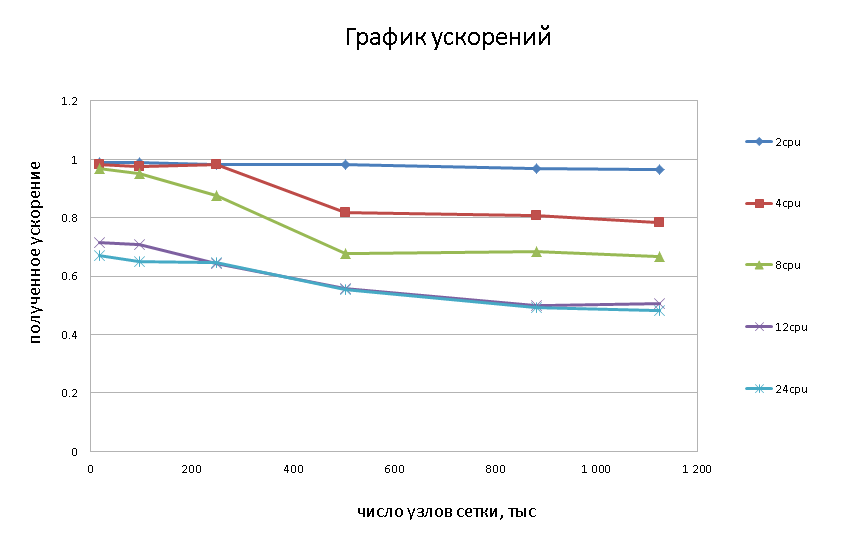
\includegraphics[width=15cm]{scpu.png} 
\caption{��������� ���������� � ����������� �� ����� ��������� ���� ����� ��� ������� ���������� �����������}\label{graph1}
\end{figure}
\begin{figure}[!h]\center
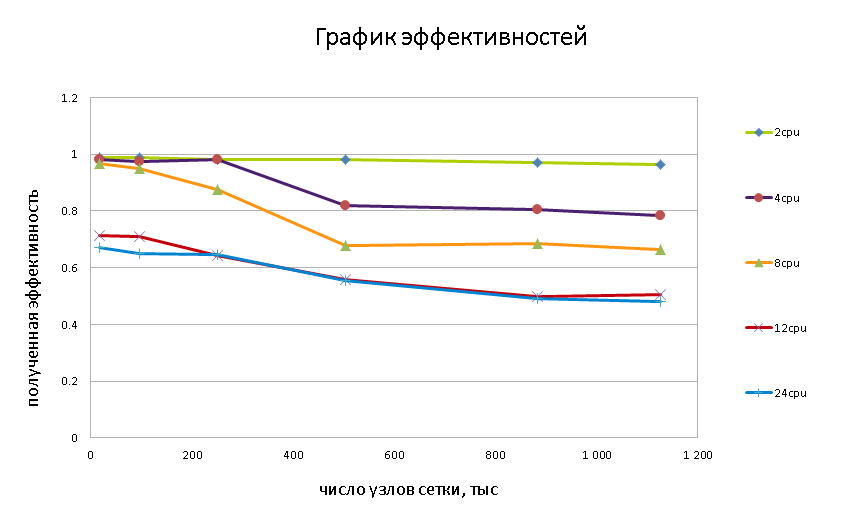
\includegraphics[width=15cm]{Effcpu.png} 
\caption{������������� ���������� � ����������� �� ����� ��������� ���� ����� ��� ������� ���������� �����������}\label{graph2}
\end{figure}

���� ������������� ��� ���������� ����� ����������� ���������� ������������
������ ����� ����� �����, ���������� ������ ����� �������������.
�������� ����� ���� �������� ���������� ������� �� ���� ������������ ����
���������, ��� ����������� ������� � ����������.

\subsubsection{���������� ����������� ���������� ��������� CUDA � MPI}
�� ����� ���������� �������� �-100 ������������ ������� ���������� ����� 6.2 ��� �����
��������� �����. �� ��������� ������ ����� ��� �������� �� ����� ���������� ��������� ���������� 
������� 30 ���. ���������� ��������� ������� �������� ��� ������������� �������������
���������� ��������� ��� ��������� ������ ������� � ������. ����� ��������� ����������
������������ ����� ��������-�������� ������ � GPU �� CPU � ����� ������� ����� CPU � ������� MPI.
�� ����������� ������� (���.~\ref{graph3}) ����������
��������� ���������� � ����������� �� ����� ��������� ���� �����. ������� �������� �� 
������� ������������� �� 1 �� 6 ����������� ����, ��������������.
\begin{figure}[!h]\center
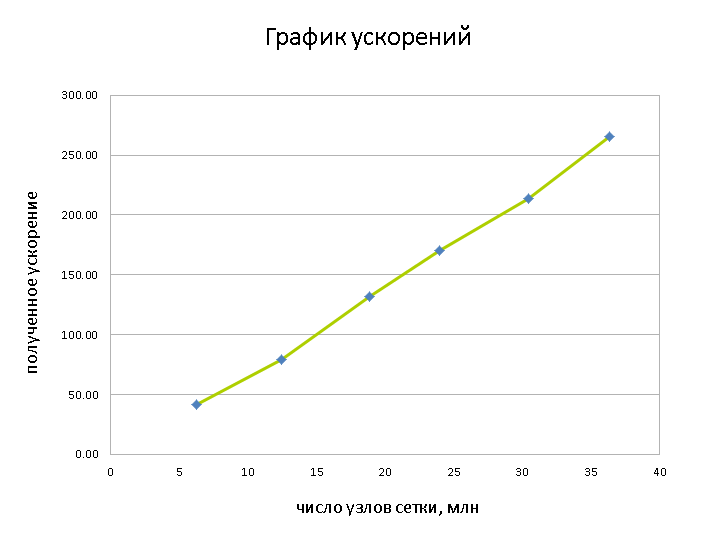
\includegraphics[width=16cm]{sgpu.png} 
\caption{��������� ���������� � ����������� �� ���������� ����� ��������� �������(����� ����������� ����������� �������� �� ����� � ����� -- �� 1 �� 6).}\label{graph3}
\end{figure}

����� �������, � ���������� ������������� �������� � ��������� ������������ ����
�������� ��������� � 265 ���, ��� ���� �� �-100 ���� ������������� ��� ��������� ���� 
�� ��������� 64 ��� ���������� �������� �� ����� �� 36��� �����(�� ����� ����
���������� 12CPU � 3GPU).
���������� ���������� ��������� ������������, ��� ����� ������������ ���������
�������� �������� ������� � ������������ ����� �������� ����� �������
�������������� �����.
\section{Заключение}

В процессе работы над дипломом:

\begin{itemize}
	\item 	предложены 1D, 2D и 3D-модели течений в пористых средах,
	допускающие реализацию явными численными методами;

	\item поставлены и решены модельные задачи просачивания в однородной 
	пористой среде;

	\item разработан алгоритм расчета;
	
	\item алгоритм распараллелен;
	
	\item написан программный комплекс на языке программирования C/C++ с использованием 
	библиотек MPI, CUDA для решения задач трехфазной неизотермической фильтрации;
	
	\item в необходимом на данном этапе объеме освоена технология 
	программирования на графических платах Nvidia CUDA;

	\item освоены технологии визуализации данных расчетов;

	\item программный комплекс протестирован на нескольких тестовых задачах 
	фильтрации;
	
	\item сделаны три доклада на конференциях~\citemy{MIPT-54,MIPT-55,Pareng-2013}, одна из которых -- международная~\citemy{Pareng-2013};

	\item написаны в соавторстве две статьи~\citemy{CSE,Mathmod-2014};
\end{itemize}


\makeatletter
\renewcommand{\@biblabel}[1]{#1.\hfil}
\makeatother
\addto\captionsrussian{\def\refname{Список литературы}}
\addcontentsline{toc}{section}{Список литературы}
\nocite{*}
\bibliographystyle{utf8gost705u} % ГОСТ + поправка (инициалы, потом фамилии)
\bibliography{kbib-utf8}


\end{document}
